
\section{Strontium}
\label{bursts:sec:sr}
\subsection{Nucleosynthesis}
\label{bursts:sec:sr_nuc}

\begin{figure} % fig 4
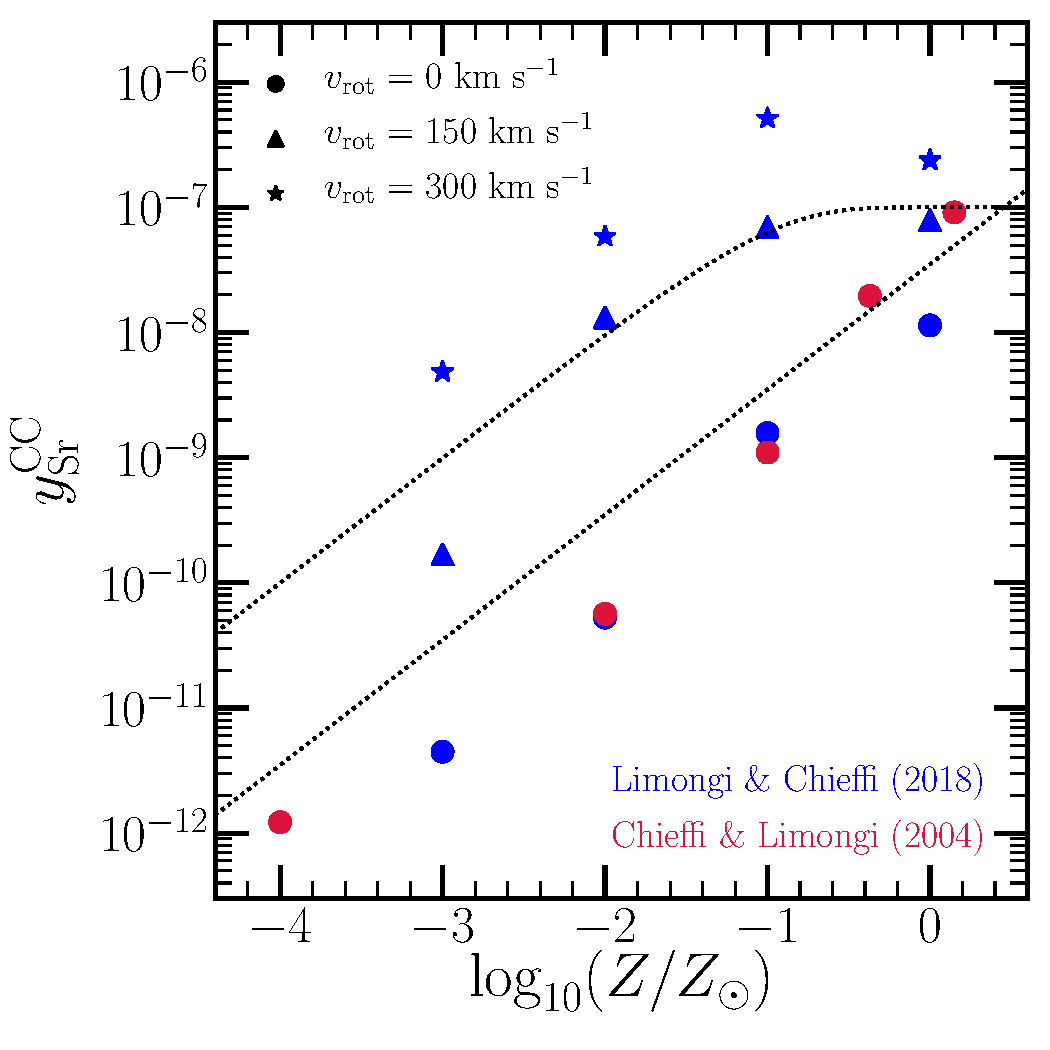
\includegraphics[scale = 0.45]{sr_cc_yields.pdf}
\caption{
IMF-averaged CCSN yields of Sr computed using the non-rotating progenitor 
models of (\citealp{Chieffi2004}, red circles) and the models 
of~\citet{Limongi2018} for progenitors with $v_\text{rot} = 0$ (blue circles), 
150 km s$^{-1}$ (blue triangles), and 300 km s$^{-1}$ (blue stars). Dotted 
curves show approximate characterizations of these results used in our GCE 
models, $y_\text{Sr}^\text{CC} = 3.5\times10^{-8}(Z/Z_\odot)$ and 
$y_\text{Sr}^\text{CC} = 10^{-7}(1 - \exp{(-10Z/Z_\odot)})$. We adopt $Z_\odot$ = 
0.014 based on~\citet{Asplund2009}. 
}
\label{bursts:fig:sr_cc_yields}
\end{figure} 

\begin{figure*} % fig 5
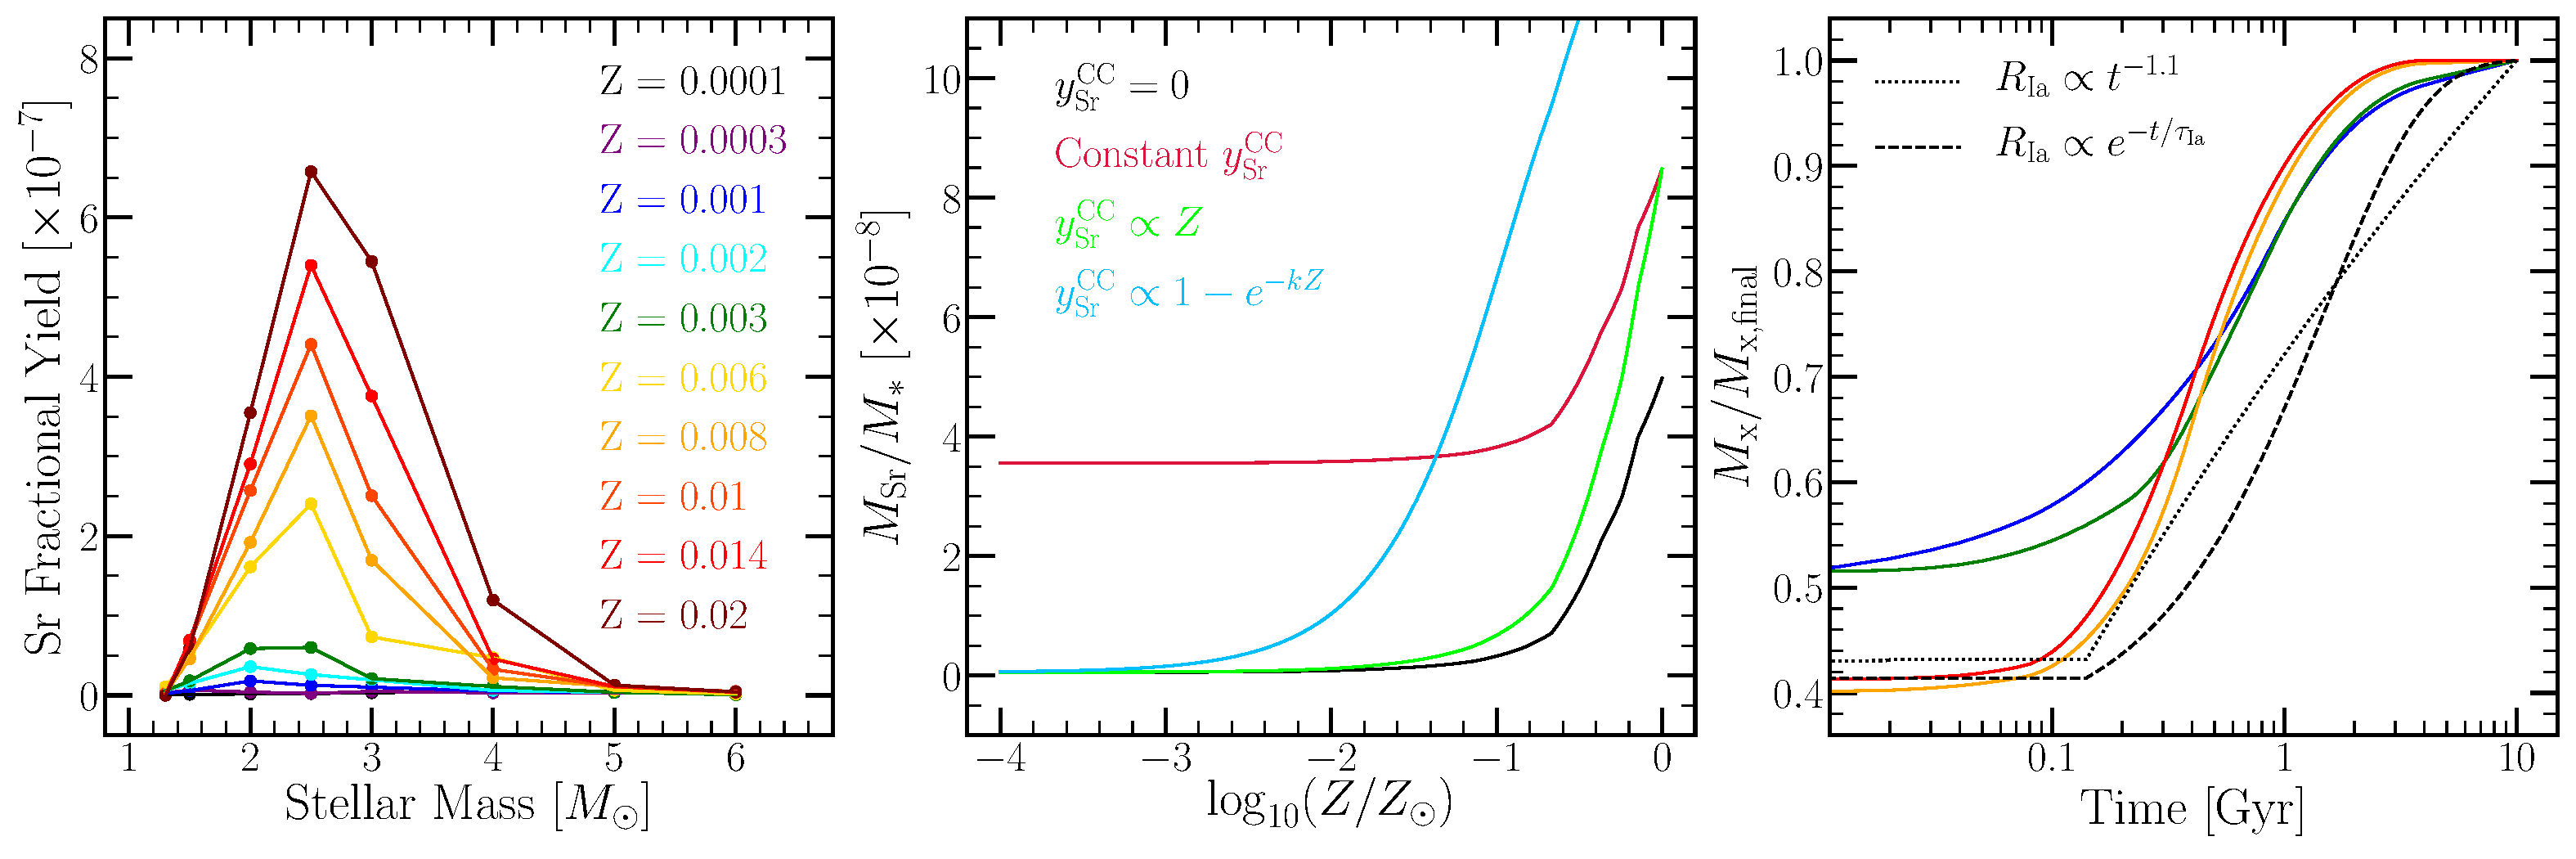
\includegraphics[scale = 0.32]{sr_yields_ssp.pdf}
\caption{
Yields of Sr as a function of stellar mass, metallicity, and time. 
\textbf{Left}: Fractional yields of AGB stars - the ejected Sr mass divided by 
the initial stellar mass, computed as a function of stellar mass and 
metallicity using the FRANEC code~\citep{Cristallo2011}. \textbf{Middle}: 
IMF-averaged Sr yield after 10 Gyr, for a single stellar population of 
metallicity $Z$ formed at $t = 0$, computed by adding the AGB yields to CCSN 
yields illustrated by the dotted curves in Fig.~\ref{bursts:fig:sr_cc_yields}, or to 
constant yields $y_\text{Sr}^\text{CC} = 3.5\times10^{-8}$ or 
$y_\text{Sr}^\text{CC} = 0$ (AGB only). \textbf{Right}: Time evolution of Sr 
production for single stellar populations of metallicity $Z$ = 0.001, 0.003, 
0.008, and 0.014, assuming the $y_\text{Sr}^\text{CC} \propto Z$ model. 
Curves are color-coded to the legend in the left panel. All curves are 
normalized to the final Sr mass produced after 10 Gyr, which depends strongly 
on $Z$ as shown in the right panel. Dotted and dashed black curves show the 
time evolution of Fe for our standard values of $y_\text{Fe}^\text{CC}$ and 
$y_\text{Fe}^\text{Ia}$ and a $t^{-1.1}$ or $e^{-t/1.5\text{ Gyr}}$ DTD with a 
minimum delay time of 0.15 Gyr. Because AGB production is dominated by 
$2-4\ M_\odot$ stars, AGB Sr enrichment from a single stellar population 
occurs faster than SN Ia Fe enrichment.  
}
\label{bursts:fig:sryields_3panel}
\end{figure*}

Strontium is one of the commonly used tracers of s-process nucleosynthesis in 
AGB stars~\citep[e.g.][]{Conroy2013a, Mishenina2019}. Sr production differs from 
that of O and Fe, the two elements that we have examined thus far, because the 
delay time of AGB enrichment differs from that of SNe Ia and because the Sr 
yields of both CCSNe and AGB stars are expected to depend strongly on 
metallicity. Both of these differences have an important impact on predicted 
evolutionary tracks and element ratio distributions. 
\par 
Fig.~\ref{bursts:fig:sr_cc_yields} plots IMF-averaged net CCSN yields of strontium 
based on the models of~\citet{Chieffi2004} and~\citet{Limongi2018}. 
These are the solutions to equation~\refp{bursts:eq:frac_yield} with the 
same IMF parameters discussed in~\S~\ref{bursts:sec:ccsne}.


\citet{Chieffi2004} report Sr yields for non-rotating CCSN progenitors 
($v_\text{rot}$ = 0) at a wide range of metallicities, while \citet{Chieffi2013} 
report yields for $v_\text{rot}$ = 0 and 300 km s$^{-1}$ but at only solar 
metallicity. Progenitor rotation affects Sr yields from CCSNe due to 
rotationally induced mixing~\citep{Frischknecht2016}. We presume the results 
of~\citet{Chieffi2013} to be superseded by those of~\citet{Limongi2018}, who 
examined a range of metallicites and values of $v_\text{rot}$ = 0, 150 km 
s$^{-1}$, and 300 km s$^{-1}$. However, we caution that the impact of rotation 
on the Sr yield at solar metallicity is much stronger in 
the~\citet{Limongi2018} study than in~\citet{Chieffi2013} due to a different 
calibration of the rotation-induced mixing efficiency. 
\par 
Fig.~\ref{bursts:fig:sr_cc_yields} shows that the predicted CCSN yields depend 
strongly on metallicity and are much higher (typically 1-3 orders of magnitude) 
for rapidly rotating vs. non-rotating progenitors. As approximate descriptions 
of the numerical results, we show the functions 
\begin{subequations}\begin{align} 
y_\text{Sr}^\text{CC} &= 3.5\times10^{-8}(Z / Z_\odot) 
\label{bursts:eq:y_sr_cc_linear} \\ 
\intertext{for v$_\text{rot}$ = 0 and} 
y_\text{Sr}^\text{CC} &= 10^{-7}\left[1 - e^{-10(Z/Z_\odot)}\right] 
\label{bursts:eq:y_sr_cc_limexp} 
\end{align}\end{subequations} 
for $v_\text{rot}$ = 150 km s$^{-1}$. For comparison, we will also compute GCE 
models with a constant $y_\text{Sr}^\text{CC} = 3.5\times10^{-8}$ matched to 
our linear model at $Z = Z_\odot$ and with $y_\text{Sr}^\text{CC} = 0$ 
corresponding to pure AGB enrichment. We caution that these are not fits to 
the yields plotted in Fig.~\ref{bursts:fig:sr_cc_yields}; we adopt them as an 
agnostic approach to the form of the metallicity-dependent yield in the 
interval -2 $\lesssim$ [Fe/H] $\lesssim$ 0 in which our models are focused. 
\par
For AGB production of Sr, we use fractional yields as a function of initial 
stellar mass at various metallicities from the FRANEC 
code~\citep{Cristallo2011}. These are plotted in the left-hand panel of 
Fig.~\ref{bursts:fig:sryields_3panel}, and they show two notable features. First, 
for near-solar metallicity the fractional yields are sharply peaked at stellar 
masses of 2-3 $M_\odot$. To obtain the total mass yield per star one 
multiplies by $M$, giving weight to the contribution of higher mass 
stars, but the number of stars per linear $\Delta M$ interval is proportional 
to $M^{-2.3}$ for a Kroupa IMF in this mass range, thus increasing the weight 
of lower mass stars. The strong mass dependence of the fractional yields means 
that the IMF-averaged AGB yield is dominated by stars with relatively short 
lifetimes. The second notable feature is a strong metallicity dependence, 
expected because the amount of Sr produced via the s-process during the AGB 
phase should increase with the abundance of free neutrons produced by nuclear 
reactions involving C and Ne isotopes. For $Z\lesssim Z_\odot/3$ the predicted 
fractional yields are below $10^{-7}$ at all masses, and for 
$Z\gtrsim Z_\odot/3$ the maximum fractional yield is roughly proportional to 
$Z$. 
\par 
In the middle panel of Fig.~\ref{bursts:fig:sryields_3panel}, the black curve shows 
the late-time ($t = 10$ Gyr), IMF-averaged AGB Sr yield as a function of 
metallicity. At $Z = Z_\odot$, the yield is $y_\text{Sr}^\text{AGB} = 
5\times10^{-8}$, but for $Z < Z_\odot/3$ the yield is well below $10^{-8}$. 
The green curve shows the total yield from adding $y_\text{Sr}^\text{AGB}$ to 
the $y_\text{Sr}^\text{CC}$ of equation~\refp{bursts:eq:y_sr_cc_linear}, which 
approximates the non-rotating~\citet{Limongi2018} models. At all metallicities 
for which $y_\text{Sr} > 10^{-8}$, the CCSN and AGB contributions are 
comparably important. However, for the $v_\text{rot} = 150\text{ km s}^{-1}$ 
yields approximated by equation~\refp{bursts:eq:y_sr_cc_limexp}, the CCSN yields 
dominate over the AGB yields at all metallicities (blue curve). The red curve 
shows the simple case of adding $y_\text{Sr}^\text{AGB}$ to a constant 
$y_\text{Sr}^\text{CC} = 3.5\times10^{-8}$. 

\begin{figure*} % fig 6 
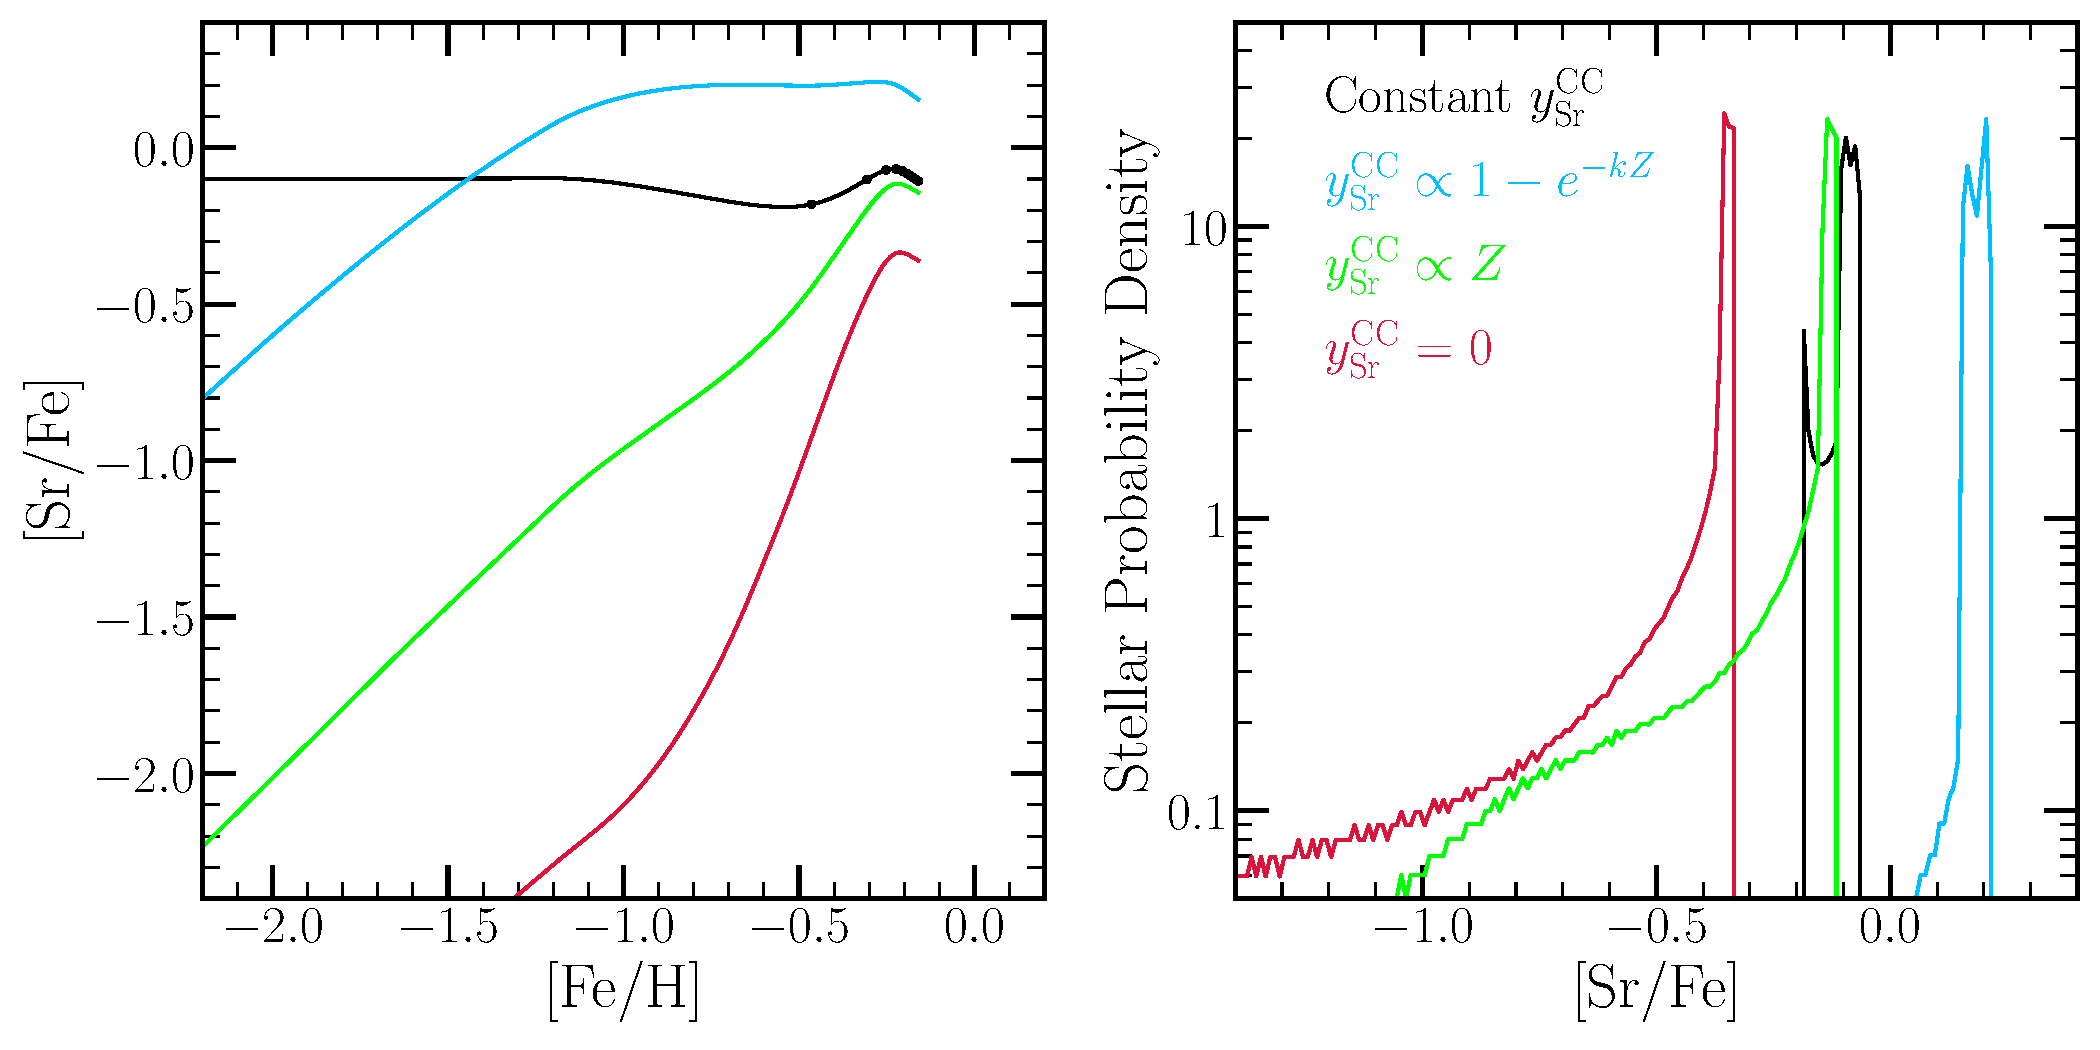
\includegraphics[scale = 0.45]{sr_yield_assumptions.pdf}
\caption{
Evolutionary tracks (left) and final [Sr/Fe] distributions (right) under our 
fiducial burstless GCE model for four different assumptions about 
$y_\text{Sr}^\text{CC}$: constant yield, zero yield, and the 
metallicity-dependent yields for non-rotation or rotation progenitors 
described by equations~\refp{bursts:eq:y_sr_cc_linear} and~\refp{bursts:eq:y_sr_cc_limexp}. 
The red ($y_\text{Sr}^\text{CC} = 0$) curve shows the predicted evolution for 
our metallicity dependent AGB yields (\citealp{Cristallo2011}; 
Fig.~\ref{bursts:fig:sryields_3panel}), which are adopted in all four models. On the 
black curve, small black points are plotted at $\Delta t$ = 1 Gyr intervals, 
and all models reach a given [Fe/H] at the same time. 
}
\label{bursts:fig:sr_yields}
\end{figure*}

The right panel of Fig.~\ref{bursts:fig:sryields_3panel} shows the time evolution of 
Sr production for a selection of metallicity values shown in the left panel, 
$Z$ = 0.001, 0.003, 0.008, and 0.014. All curves are normalized by the 
late-time yield, which is strongly dependent on metallicity as shown in the 
middle panel. Here we adopt the $y_\text{Sr}^\text{CC} \propto Z$ yield model 
for CCSNe, and in all cases this accounts for about 40-50\% of the total yield. 
Typically about half of the AGB contribution comes within the first 0.5 Gyr, 
and nearly all of it within 2 Gyr. Dotted and dashed curves show the evolution 
of Fe production for our fiducial values of $y_\text{Fe}^\text{CC} = 0.0012$ 
and $y_\text{Fe}^\text{Ia} = 0.0017$ and a $t^{-1.1}$ DTD or an 
$e^{-t/1.5\text{ Gyr}}$ DTD, respectively. Although our assumed minimum delay 
is $t_\text{D} = 0.15$ Gyr, getting half of the SN Ia Fe contribution 
takes~$\sim0.9 - 1$ Gyr, so the AGB Sr enrichment is faster, albeit moderately, 
than the SN Ia Fe enrichment. This rapid AGB contribution is a consequence of 
the dominant contribution from $2 - 4\ M_\odot$ stars, which have short 
lifetimes. These curves represent the Sr production from a single population of 
stars at a given metallicity. In a GCE model the metallicity itself rises with 
time, thus increasing the Sr production because of the metallicity-dependent 
yield. In the next section, we demonstrate that this complicates the 
enrichment timescale of Sr relative to Fe. 

\begin{figure*} % fig 7
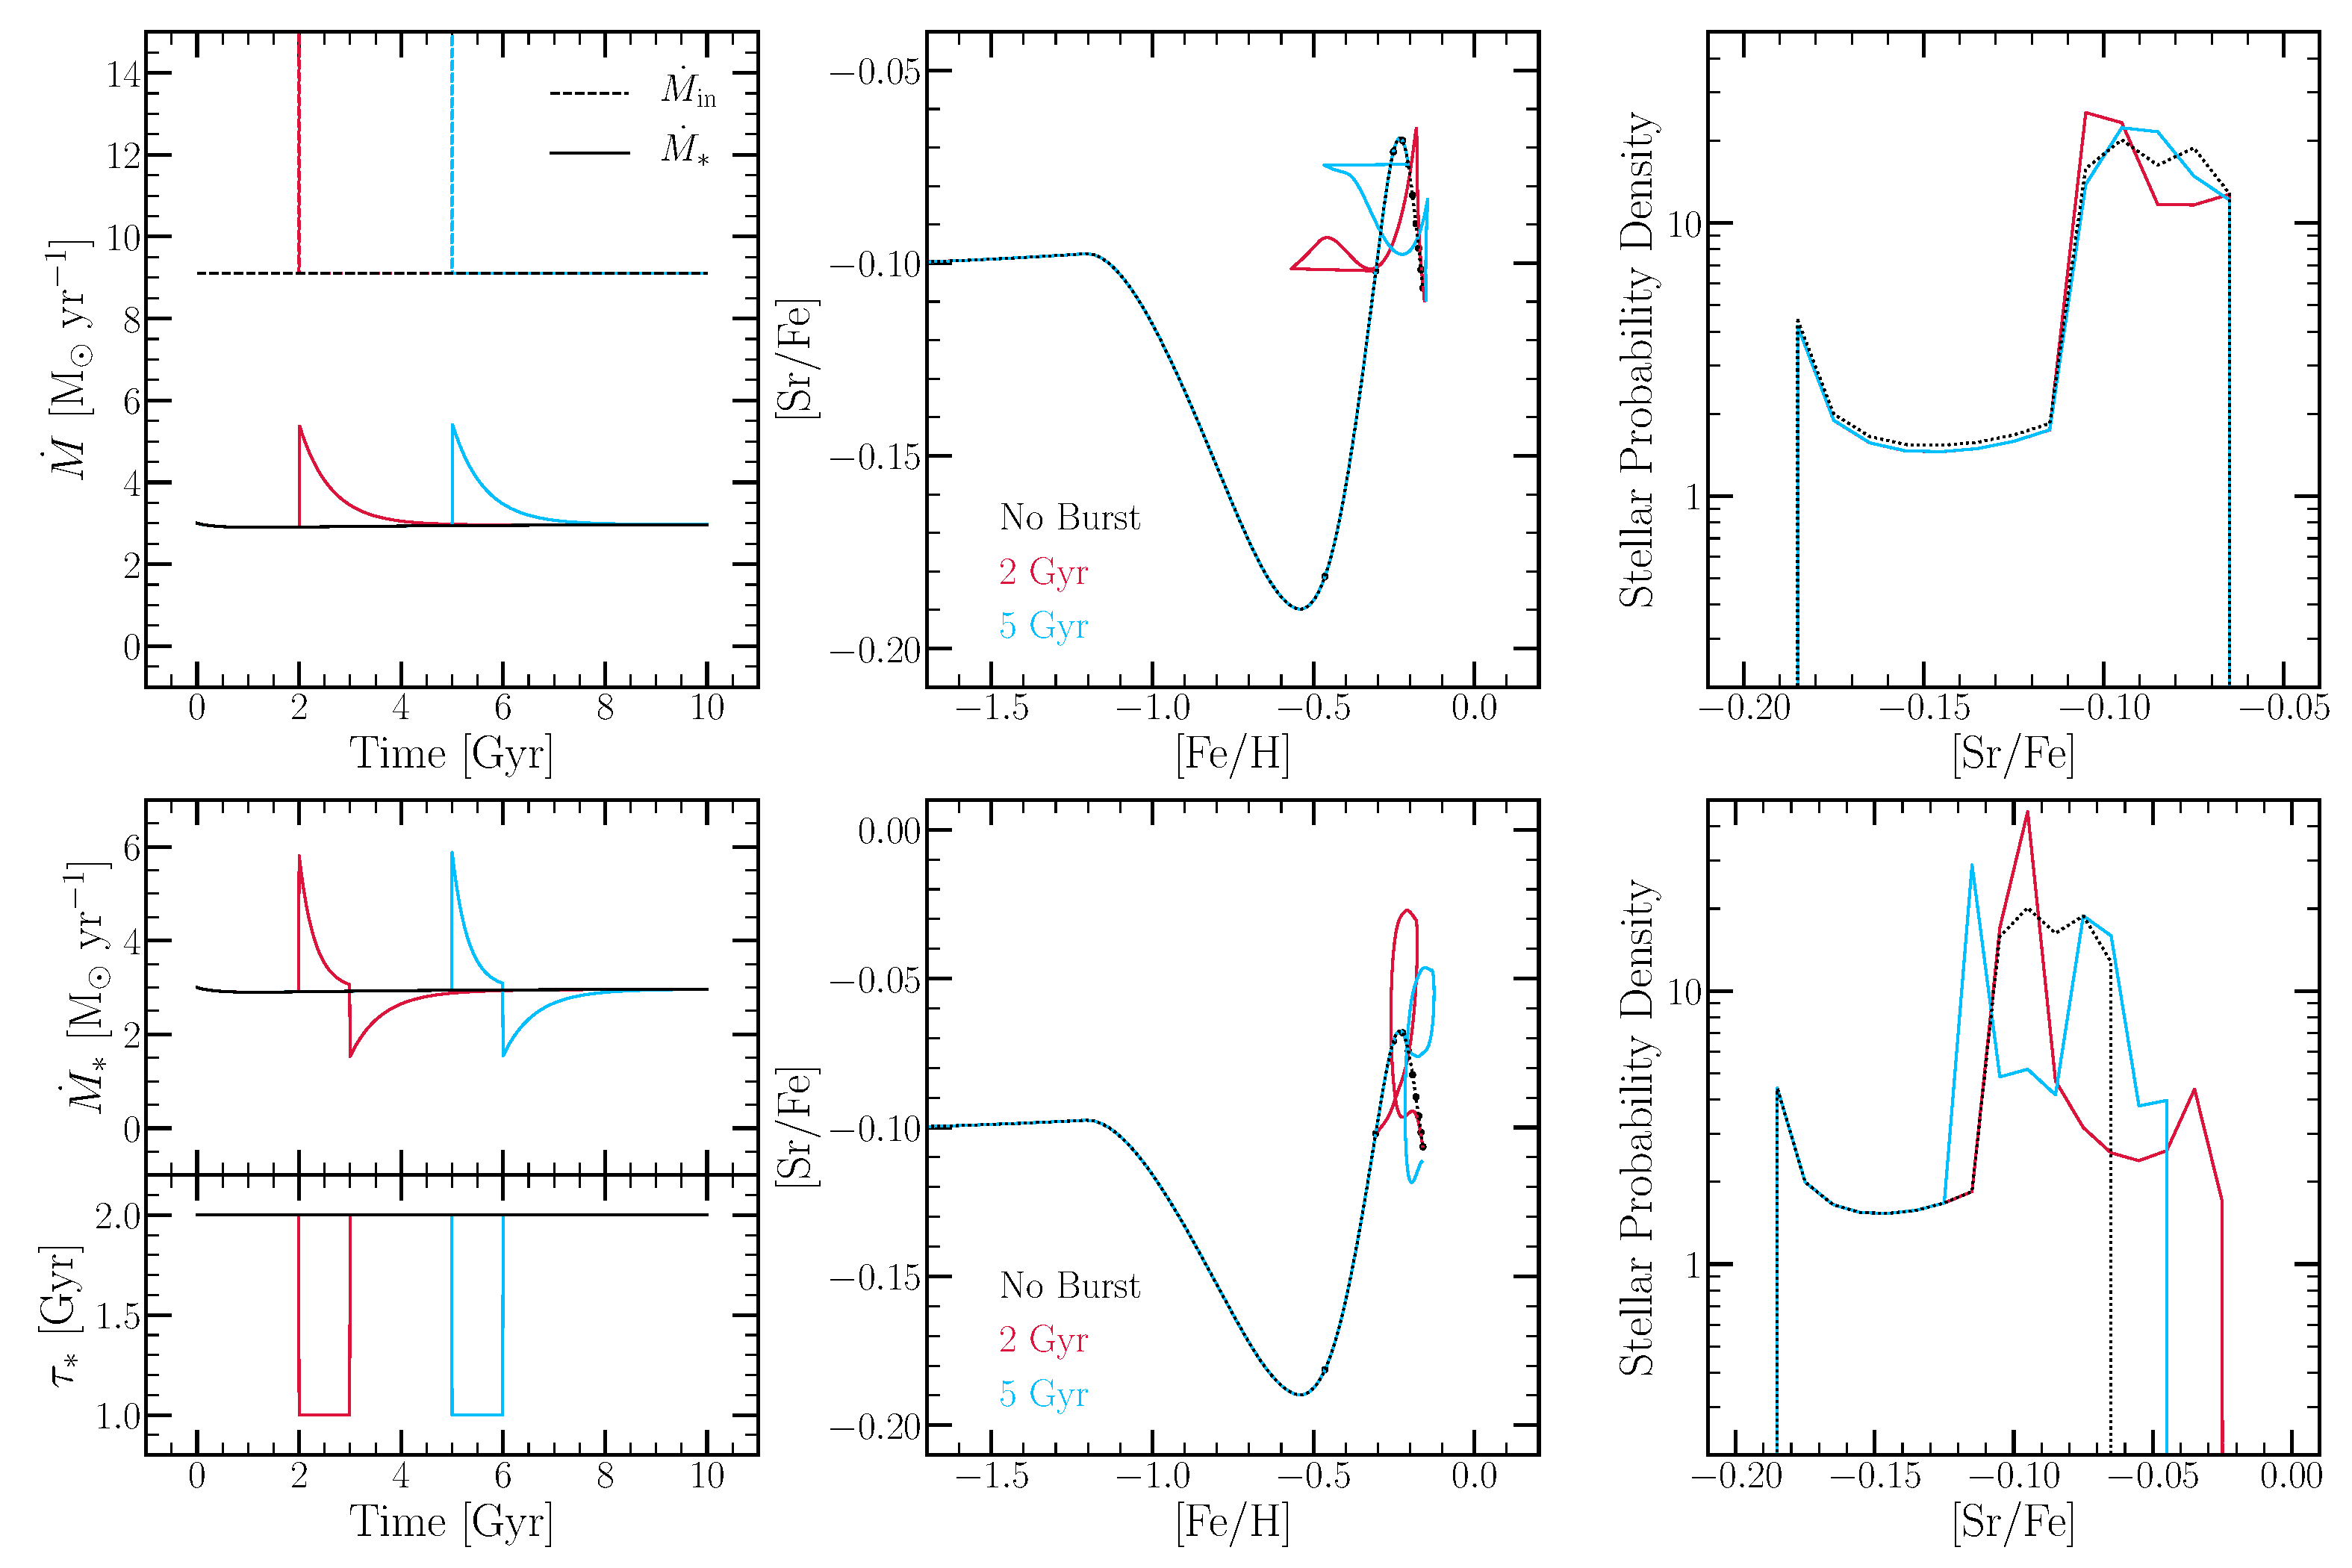
\includegraphics[scale = 0.31]{fiducial_bursts_sr.pdf}
\caption{
Evolutionary tracks (middle) and final [Sr/Fe] distributions (right) for our 
fiducial starburst models, analogous to the top and bottom rows of 
Fig.~\ref{bursts:fig:fiducial_cases}. All models adopt $y_\text{Sr}^\text{CC} = 
3.5\times10^{-8}$ and the~\citet{Cristallo2011} AGB yields illustrated in 
Fig.~\ref{bursts:fig:sryields_3panel}. 
}
\label{bursts:fig:bursts_srfe}
\end{figure*}

\subsection{Smooth Evolution}
\label{bursts:sec:sr_enrich} 

Fig.~\ref{bursts:fig:sr_yields} shows the [Sr/Fe]-[Fe/H] tracks and [Sr/Fe] 
distributions for our fiducial unperturbed GCE model, with constant SFR, 
$\tau_* = 2$ Gyr,~$\eta = 2.5$, and the AGB Sr yields illustrated in 
Fig.~\ref{bursts:fig:sryields_3panel}. We consider four different assumptions about 
CCSN yields: $y_\text{Sr}^\text{CC} = 0$, $y_\text{Sr}^\text{CC} = 
3.5\times10^{-8}$, and the metallicity dependent yields of 
equations~\refp{bursts:eq:y_sr_cc_linear} and~\refp{bursts:eq:y_sr_cc_limexp}. The 
$y_\text{Sr}^\text{CC} = 3.5\times10^{-8}$ model has a flat plateau at 
[Sr/Fe] = -0.1 for [Fe/H] $< -1.0$, which reflects the ratio of our constant 
CCSN yields. The [Sr/Fe] ratio then dips downward as SN Ia Fe enrichment 
becomes important, analogous to the knee in [O/Fe]-[Fe/H] evolution. However, 
as [Fe/H] rises further, AGB enrichment becomes competitive with CCSN 
enrichment, and [Sr/Fe] moves upward. After reaching a maximum at [Fe/H] = 
-0.2, [Sr/Fe] = -0.1, the [Sr/Fe] curves turns downward again because the 
timescale of SN Ia enrichment is longer than that of AGB enrichment. Even 
though single stellar populations generally produce Sr before Fe (see 
Fig.~\ref{bursts:fig:sryields_3panel}), the bulk of the Sr production in GCE follows 
the bulk production of more abundant elements like O and Fe due to the 
metallicity dependence of the yields. The [Sr/Fe] distribution of this model 
has a peak at [Sr/Fe]$\approx$-0.18, corresponding to the minimum in the 
[Sr/Fe]-[Fe/H] curve, and a second, higher peak at [Sr/Fe]$\approx$-0.1. In 
detail, this second peak is split in two, corresponding to the maximum in the 
[Sr/Fe]-[Fe/H] track and the slightly lower final equilibrium. 
\par 
With $y_\text{Sr}^\text{CC} = 0$ (AGB only), the [Sr/Fe] ratio is below -2 for 
[Fe/H] $<$ -1 and rises steeply with increasing [Fe/H], reaching a maximum at 
[Sr/Fe]$\approx$-0.35. Adding CCSN enrichment with $y_\text{Sr}^\text{CC} 
\propto Z$, corresponding approximately to the non-rotating~\citet{Limongi2018} 
yields, gives a shallower but still steeply rising [Sr/Fe]-[Fe/H] trend, which 
peaks at [Sr/Fe]$\approx$-0.1. Although one can see the imprint of SN Ia Fe 
enrichment on both of these curves, it is subtle relative to the strong trend 
arising from metallicity-dependent CCSN yields. 
\par 
Our approximate model of the rotating~\citet{Limongi2018} yields given by 
equation~\refp{bursts:eq:y_sr_cc_limexp} produces a [Sr/Fe] curve that rises rapidly 
until [Fe/H] = -1, then stays nearly constant at [Sr/Fe]$\approx$+0.2. AGB 
enrichment is small relative to CCSN enrichment in this model, as shown in 
Fig.~\ref{bursts:fig:sryields_3panel}. There is still a slight dip in [Sr/Fe] at 
late times, producing a split in the [Sr/Fe] distribution. 
\par 
Spectra of early-type galaxies imply [Sr/Fe]$\approx$0 for stellar populations 
typically dominated by solar or mildly super-solar 
metallicities~\citep{Conroy2013a}, showing that solar abundance ratios arise 
even in systems with very different star formation histories from the Milky 
Way. Measurements of individual stars in the Milky Way and in dwarf satellites 
show median trends that are roughly flat at [Sr/Fe]$\approx$0 down to 
[Fe/H]$\approx$-3, though the star-to-star scatter becomes large below 
[Fe/H] = -1~\citep[see, e.g.,][and references therein]{Mishenina2019, 
Hirai2019}. Above [Fe/H] = -1, our model with the~\citet{Limongi2018} rotating 
CCSN progenitor yields produces a flat [Sr/Fe] trend, but only our 
$y_\text{Sr}^\text{CC}$ = constant model produces a flat trend to [Fe/H] as low 
as -3. We conclude that reproducing Milky Way observations requires an 
additional source of Sr that is prompt compared to SN Ia enrichment and 
approximately independent of metallicity at least for [Fe/H] $< -1$. This is 
in agreement with more detailed models of Sr enrichment investigating a 
variety of potential sources, such as neutron star mergers, electron-capture 
and magnetorotationally driven supernovae, and rotating massive 
stars~\citep[e.g.][]{Cescutti2014, Cescutti2015, Prantzos2018, Hirai2019, 
Rizzuti2019}. Neutron-rich neutrino-driven winds from newly 
formed neutron stars should also produce Sr via r-process nucleosynthesis in 
core collapse supernovae~\citep{Thompson2001,Vlasov2017,Thompson2018}, and 
this production is typically not included in calculations of CCSN yields such 
as~\citet{Limongi2018}. Sources that produce relatively large amounts of Sr in 
events that are individually rare would help to explain the large star-to-star 
scatter at low [Fe/H]. We conclude that our constant $y_\text{Sr}^\text{CC} = 
3.5\times10^{-8}$ model could retroactively account for this contribution; 
this arises from the nature of equation~\refp{bursts:eq:mdot_ccsne} which in principle 
could fold all prompt enrichment components into $y_\text{Sr}^\text{CC}$ as a 
function of metallicity. Nonetheless, we encourage caution that sufficiently 
accurate modeling of Sr production at metallicities as low as [Fe/H] $< -2$ 
may require a more complete understanding of the astrophysical origins of the 
r-process and the associated Sr yields. 



\subsection{Burst Scenarios}

Fig.~\ref{bursts:fig:bursts_srfe} shows [Sr/Fe] evolution and [Sr/Fe] distributions 
for our fiducial gas-driven and efficiency-driven starbursts, which can be 
compared to the [O/Fe] result in the top and bottom rows of 
Fig.~\ref{bursts:fig:fiducial_cases}. For ease of interpretation we have used the 
$y_\text{Sr}^\text{CC} = 3.5\times10^{-8}$ model for CCSN yields, and the 
black curves representing the unperturbed model are the same as the black 
curves in Fig.~\ref{bursts:fig:sr_yields} but shown with a zoomed-in axis range. 
In the gas-driven models, dilution with pristine gas first drives [Fe/H] lower 
at fixed [Sr/Fe]. For the burst at $t = 2$ Gyr, this backward jump is followed 
by a small upward hook, reminiscent of the behaviour of this model in [O/Fe]. 
However, this burst occurs very near the [Sr/Fe] ratio associated with the 
adopted CCSN yields, suggesting that CCSNe associated with the burst do not 
significantly modify the ISM [Sr/Fe]. Instead, it is likely that this increase 
is due to Sr production in AGB stars from earlier epochs. Subsequently, the 
detailed shape of the trajectory becomes complex as both SN Ia and AGB 
enrichment with metallicity dependent yields become important, and eventually 
it rejoins the trajectory of the unperturbed model. 
\par 
The $t = 5$ Gyr burst occurs after the maximum [Sr/Fe], produced because a 
$t^{-1.1}$ SN Ia DTD produces Fe on timescales longer than AGB stars produce 
Sr. In this model, [Sr/Fe] initially evolves downward following the addition 
of zero metallicity gas, both because of these late SNe Ia from previous 
generations of stars and because this is in the direction of the CCSN ratio of 
[Sr/Fe]$\approx$-0.1. Unfortunately, all of these excursions are small, and 
the impact on [Sr/Fe] distributions is almost negligible. Detecting the 
signature of these complex tracks would require correlating precise [Sr/Fe] 
and stellar age measurements. 
\par 
The impact of efficiency-driven bursts (lower panels) is somewhat stronger. 
Here the bursts drive upward excursions in [Sr/Fe] because both the CCSN and 
AGB channels contribute Sr faster than SN Ia Fe, and the slight boost of [Fe/H] 
increases the AGB yield. As seen previously in [O/Fe], the suppressed SFR after 
$\tau_*$ returns to its original value causes a downward hook in [Sr/Fe], as 
SN Ia Fe from stars produced during the burst dominates over the reduced CCSN 
and AGB contributions. These models produce larger deviations in the [Sr/Fe] 
distributions than the gas-driven models, with peaks at higher and lower 
[Sr/Fe] associated with the mid-burst maximum and post-burst minimum. However, 
the separation between these peaks is below 0.1-dex, so precise measurements 
would be needed to detect this signature. 
\par 
The interpretation of Fig.~\ref{bursts:fig:bursts_srfe} is complicated partly by the 
fact that three enrichment processes are involved: CCSN, SN Ia, and AGB. 
Fig.~\ref{bursts:fig:sro_bursts} examines trajectories of [Sr/O] vs. [O/H], which are 
independent of SN Ia, at least given our assumption that SN Ia yields of O and 
Sr are insignificant. Here we show trajectories for our two 
metallicity-dependent CCSN yield models as well as the constant yield model. 
Tracks with smooth star formation (left panel) resemble the [Sr/Fe]-[Fe/H] 
tracks in Fig.~\ref{bursts:fig:sr_yields}, but without the dips coming for SN Ia Fe. 
For a gas-driven burst at $t = 5$ Gyr (middle panel), trajectories jump to 
lower [O/H] through dilution, then loop downward because the burst initially 
raises the rate of CCSN relative to AGB enrichment. These loops are analogous 
to the upward loops of [O/Fe], but O is now in the ratio denominator, and 
the timescales are CCSN vs. AGB rather than CCSN vs. SN Ia. The loop is flatter 
for the rotating star yield model because AGB stars make a smaller fractional 
contribution to Sr enrichment, and the CCSN contribution is boosted for both 
Sr and O during the burst. All trajectories eventually return to the late-time 
equilibrium of the unperturbed model. 
\par 
For an efficiency-driven burst at $t = 5$ Gyr (right panel), evolutionary 
tracks have a ``balloon-on-string'' appearance that can be understood as 
follows. By the time of the burst, the oxygen abundance has evolved to 
equilibrium, with 
\begin{equation} 
\label{bursts:eq:mdot_o_eq} 
\dot{M}_\text{O} \approx y_\text{O}^\text{CC}\dot{M}_* - 
(1 + \eta - r_\text{inst})\dot{M}_*(M_\text{O}/M_\text{ISM}) = 0 
\end{equation} 
where $M_\text{O}$ and $M_\text{ISM}$ are the oxygen and total mass in the ISM, 
respectively, and the oxygen abundance is 
\begin{equation} 
Z_\text{O,eq} = \left(\frac{M_\text{O}}{M_\text{ISM}}\right)_\text{eq} = 
\frac{y_\text{O}^\text{CC}}{1 + \eta - r_\text{inst}} 
\end{equation} 
\citep[][equations (11) and (14)]{Weinberg2017b}. Boosting the star 
formation efficiency does not initially perturb $\dot{M}_\text{O}$ from 
zero because the sources and sinks are both proportional to $\dot{M}_*$, but 
the ISM gas mass decreases because of more rapid consumption, so 
$Z_\text{O} = M_\text{O}/M_\text{ISM}$ rises. The [Sr/O] ratio drops slightly 
at first because CCSN enrichment has increased relative to AGB enrichment, but 
the increased metallicity boosts the AGB Sr yield, so [Sr/O] loops upward once 
AGB enrichment from the starburst becomes important. As the burst evolves 
further, sinks exceed sources in equation~\refp{bursts:eq:mdot_o_eq}, so the [O/H] 
ratio evolves backward to lower values because $Z_\text{O} > Z_\text{O,eq}$. 
This evolution ``overshoots'' the original [O/H] equilibrium as the gas supply 
evolves back to its original value. Lower metallicity in turn leads to a drop 
in Sr yields and [Sr/O]. Eventually all models evolve back to the original 
pre-burst equilibrium. The loop of the $y_\text{Sr}^\text{CC} \propto Z$ model 
is widest in the [Sr/O] dimension because for this model AGB and CCSN yields 
both change with metallicity, and CCSN enrichment dominates over AGB enrichment 
in the $y_\text{Sr}^\text{CC} \propto 1 - e^{-kZ}$ model. 
\par 
Figs.~\ref{bursts:fig:bursts_srfe} and~\ref{bursts:fig:sro_bursts} show that the evolution of 
an AGB s-process element can be intricate because of both the intermediate 
timescale of AGB enrichment and metallicity dependent yields. Unfortunately the 
perturbations of [Sr/Fe] and [Sr/O] ratios are relatively small, so diagnosing 
starbursts with these ratios will require precise abundance measurements 
and reasonably precise stellar ages. 

